\section{Numerical results}

\subsection{Implementation}

\subsection{Performance analysis on a large-scale instance}
We first assess the performance of each KKT solver
on a large-scale OPF instance: {\tt case9241pegase}. The model
has a total of 85,568 variables, 82,679 equality constraints and 48,147
inequality constraints, and is implemented using our package ExaModels.jl.
It is acknowledge that this particular instance is challenging to solve
with IPM, as it requires a non-trivial amount of primal-dual regularization
to achieve convergence.
Our previous work has pointed that the KKT solver is the current bottleneck
in the numerical implementation~\cite{shin2023accelerating}.

\subsubsection{Null-space strategy}
TODO

\subsubsection{Golub \& Greif strategy}
In Figure~\ref{fig:hybrid:gamma} we depict the evolution of the number
of CG iterations and accuracy, while increasing the parameter $\gamma$
from $10^4$ to $10^8$. The associated table details the time spent
in the algorithm.

On the algorithmic side, we observe that the higher the regularization $\gamma$,
the fastest the CG algorithm: we decrease the total number of iterations
spent in CG by a factor of 10. However, we have to pay a price in term
of accuracy: for $\gamma > 10^8$ the solution returned by the linear solver
is not accurate enough and the IPM algorithm has to proceed to more
primal-dual regularization, leading to an increase in the total number of iterations.

On the numerical side, the table in Figure~\ref{fig:hybrid:gamma} compares
the time spent in the IPM solver on the CPU (using CHOLMOD) and on the GPU
(using the solver {\tt cuDSS}). We observe that overall {\tt cuDSS} is
faster than CHOLMOD, leading to a decrease in the total IPM solution time.
We note that we decrease by a factor of 5 the time to assemble the condensed
matrix $K_\gamma$ on the GPU, meaning that this operation is not a bottleneck in
the algorithm.

\begin{figure}[!ht]
  \centering
  \resizebox{\textwidth}{!}{
  \begin{tabular}{|r|rrrrr|rrrrr|}
  \hline
  & \multicolumn{5}{c|}{\bf CHOLMOD (CPU)} & \multicolumn{5}{c|}{\bf cuDSS (CUDA)} \\
  \hline
  $\gamma$ & \# it & cond. (s) & CG (s) & linsol (s) & IPM (s) & \# it & cond. (s) & CG (s) & linsol (s) & IPM (s) \\
  \hline
  $10^4$ & 63 & 0.42 & 16.87 & 21.36 & 23.85 & 62 & 0.09 & 30.24 & 31.05 & 33.51 \\
  $10^5$ & 63 & 0.42 & 6.13 & 10.66 & 13.42 & 62 & 0.09 & 10.44 & 11.24 & 13.64 \\
  $10^6$ & 63 & 0.43 & 2.58 & 7.09 & 9.53 & 62 & 0.09 & 4.53 & 5.33 & 7.69 \\
  $10^7$ & 63 & 0.43 & 1.42 & 6.11 & 8.81 & 62 & 0.09 & 2.44 & 3.24 & 5.62 \\
  $10^8$ & 105 & 1.11 & 1.78 & 12.39 & 16.77 & 90 & 0.20 & 2.51 & 3.82 & 7.90 \\
  \hline
  \end{tabular}
  }
  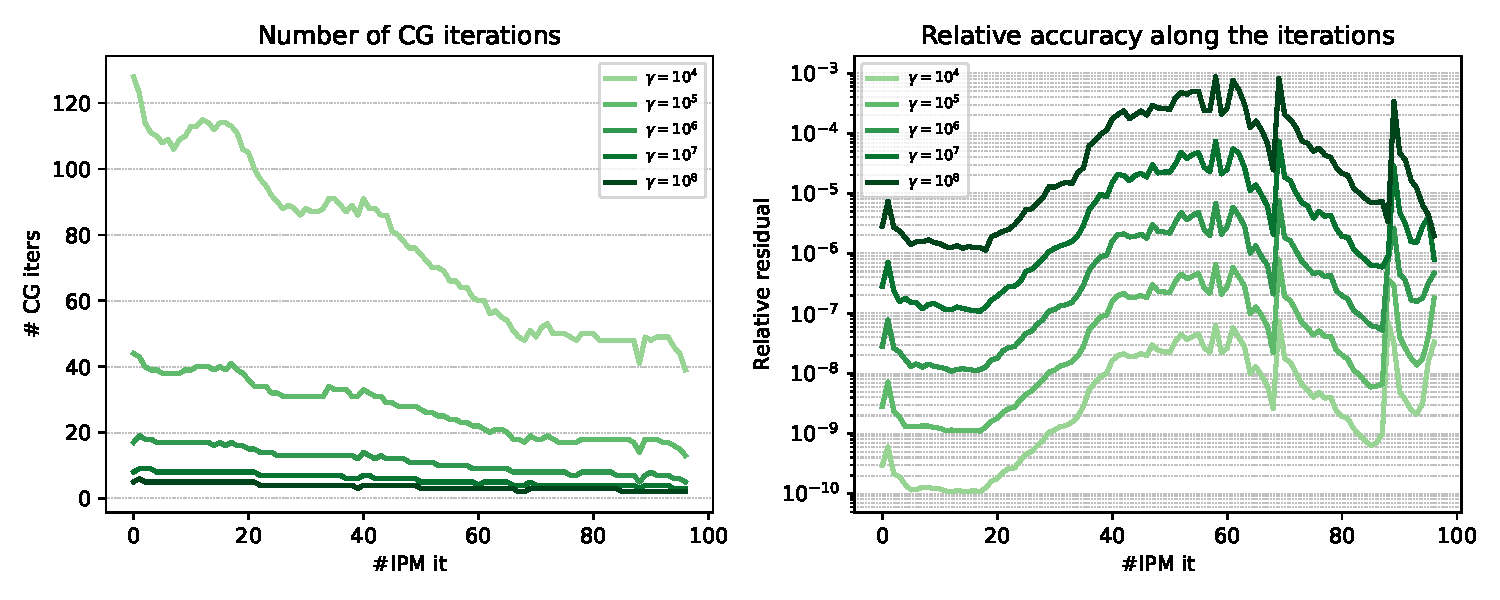
\includegraphics[width=\textwidth]{../figures/hybrid-gamma.pdf}
  \caption{
    Above: Decomposition of IPM solution time across
    (a) condensation time (cond.), (b) CG time, (c) total time
    spent in linear solver (linsol.) and (d) total time spent in
    IPM solver (IPM).
    Below: Impact of $\gamma$ on the total number of CG iterations
    and on the norm of the relative residual at each IPM iteration.
    The peak observe in the norm of the relative residual correspond
    to the primal-dual regularization performed inside the IPM algorithm,
    applied when the matrix $K_\gamma$ is not positive definite.
    \label{fig:hybrid:gamma}
  }
\end{figure}



\subsubsection{Equality relaxation strategy}
We now analyze the numerical performance of the equality relaxation strategy described in
Section~\ref{sec:kkt:sckkt}. The method solves the KKT system~\eqref{eq:kkt:condensed}
using a direct solver, as the relaxed problem does not have any equality constraints.
The parameter $\varepsilon$ used in the equality relaxation $-\varepsilon \leq g(x) \leq \varepsilon$
is set equal to the IPM tolerance $\varepsilon_{tol}$: in practice, it does not
make sense to set a parameter $\varepsilon$ below the IPM tolerance as the
inequality constraints are satisfied only up to a tolerance $\pm \varepsilon_{tol}$
in IPM.

We compare the performance obtained by the equality relaxation strategy
in Table~\ref{tab:sckkt:performance}, for different values of $\varepsilon_{tol}$.
We display both the runing times on the CPU (using CHOLMOD) and on the GPU
(using cuDSS), as well as the relative accuracy achieved as we decrease the tolerance
$\varepsilon_{tol}$: we compare the solution
returned by the equality relaxation strategy together
with the solution returned by MadNLP when running on the CPU
with HSL ma27 for a tight tolerance ($\varepsilon_{tol} = 10^{-8}$).
We observe that we cannot solve the relaxed problem in MadNLP
with a tolerance below $10^{-5}$. Indeed, the slacks associated
to the relaxed equality constraints $-\varepsilon \leq g(x) \leq \varepsilon$
are converging to a value below $2 \varepsilon$ at the optimum,
leading to highly ill-conditionned terms in the diagonal matrices
$\Sigma_s$: despite being easier to solve, the conditioning
of the relaxed problem is preventing the IPM solver to converge
to a solution more accurate than $10^{-5}$.

This observation is corroborated by the results in Table~\ref{tab:sckkt:performance}.
Overall, we observe that the method is converging fast
if the tolerance $\varepsilon_{tol}$ is above $10^{-4}$.
The method benefits from the GPU-accelerated linear solver cUDSS, as
the running time decreases by a factor of 4 compared to CHOLMOD
running on the CPU. However, the method remains inaccurate:
for $\varepsilon_{tol} = 10^{-4}$, we get a $0.5$\% error on the objective,
and a $10$\% error on the primal solution.
To achieve convergence for the lower tolerance $\varepsilon_{tol} = 10^{-5}$,
we had to decrease the tolerance of the iterative refinement
to $10^{-12}$ to get a solution accurate enough in the linear solve:
this explains the significant slowdown, as we have to perform more
backsolve per iteration thanks to the additional iterative refinement
iterations.

\begin{table}[!ht]
  \centering
  \begin{tabular}{|l|rr|rr|rr|}
    \hline
    & \multicolumn{2}{c|}{\bf CPU (CHOLMOD)} & \multicolumn{2}{c|}{\bf CUDA (cuDSS)} & \multicolumn{2}{c|}{\bf accuracy} \\
    \hline
    $\varepsilon_{tol}$ & \#it & time (s) & \#it & time (s) & $\delta_{obj}$ & $\delta_{x}$ \\
    \hline
    $10^{-2}$ & 86  & 11.7 & 86  & 1.9  & $3.4 \times 10^{-1}$ & 0.66 \\
    $10^{-3}$ & 85  & 11.7 & 85  & 1.8  & $3.9 \times 10^{-2}$ & 0.22 \\
    $10^{-4}$ & 88  & 14.1 & 86  & 2.1  & $4.1 \times 10^{-3}$ & 0.10 \\
    $10^{-5}$ & 140 & 38.0 & 184 & 11.7 & $4.6 \times 10^{-4}$ & 0.06 \\
    \hline
  \end{tabular}
  \caption{Performance of the equality-relaxation
    strategy as we decrease the IPM tolerance $\varepsilon_{tol}$.
    \label{tab:sckkt:performance}.
    The table displays the wall time on the CPU (using CHOLMOD)
    and on the GPU (using cuDSS). We display the
    relative errors on the objective $\delta_{obj} = (f(x_{hsl}^\sharp) - f(x_{sc}^\sharp))/f(x_{hsl}^\sharp)$
    and on the primal solution $\delta_x = \|x_{hsl}^\sharp - x_{sc}^\sharp\|_\infty
    / \|x_{hsl}^\sharp\|_\infty$.
  }
\end{table}


\subsubsection{Performance profile}
Now, we look at a detailed performance profile that decomposes
the total running time spent at each iteration. Using the performance
profile, we highlight the bottlenecks of each KKT solvers.

\begin{figure}[!ht]
  \centering
  \begin{minipage}{.5\textwidth}
  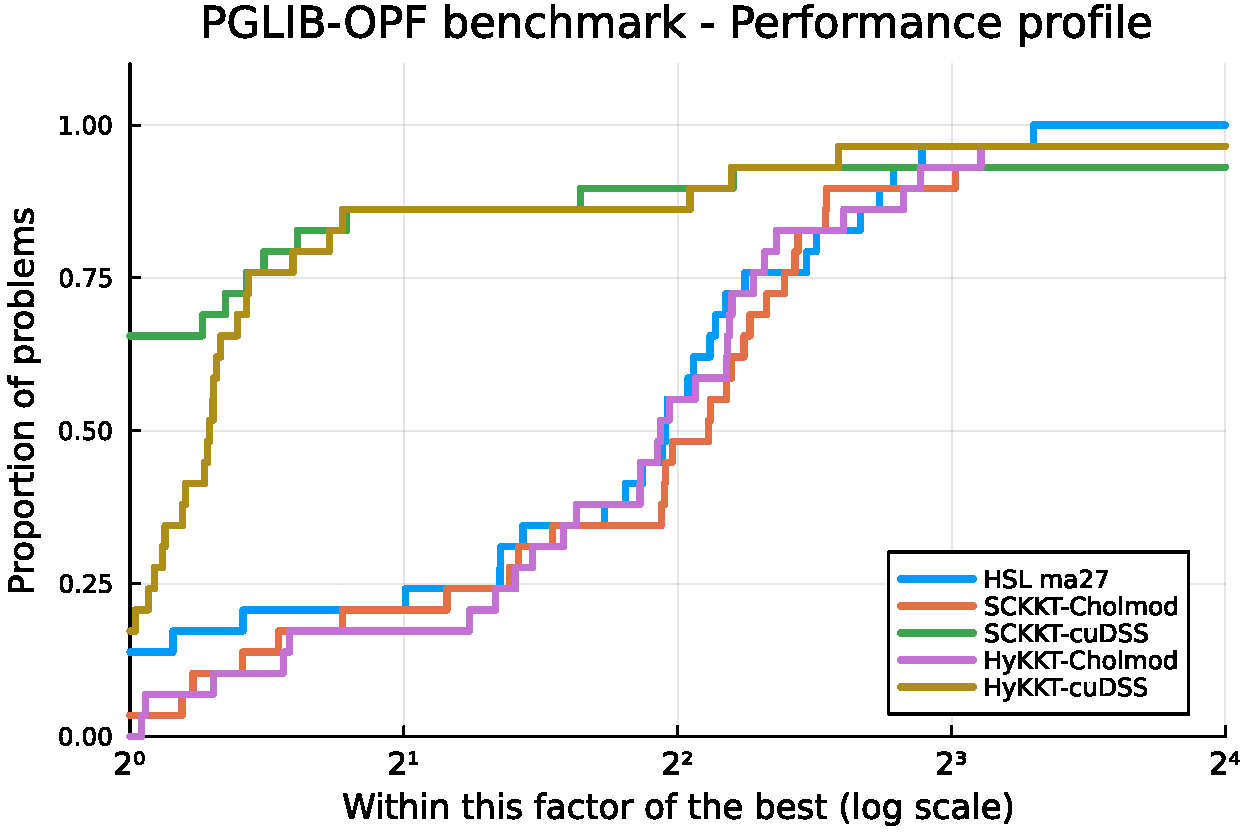
\includegraphics[width=\textwidth]{../figures/pprof.pdf} \qquad
  \end{minipage}\hfill
  \begin{minipage}{.5\textwidth}
  \resizebox{.8\textwidth}{!}{
    \begin{tabular}{lrrrr}
      \toprule
       & build & factorize & backsolve & accuracy \\
      \midrule
      hsl & 2.86e-03 & 4.78e-02 & 1.74e-02 & 7.80e-07 \\
      sckkt-cpu & 5.41e-03 & 5.05e-02 & 1.96e-02 & 1.36e-04 \\
      hckkt-cpu & 5.20e-03 & 5.10e-02 & 3.02e-02 & 3.28e-03 \\
      sckkt-cuda & 1.55e-03 & 1.81e-02 & 1.01e-02 & 8.64e-06 \\
      hckkt-cuda & 1.40e-03 & 1.43e-02 & 5.22e-02 & 2.66e-03 \\
      \bottomrule
    \end{tabular}
  }
  \end{minipage}
  \caption{Performance profile}
\end{figure}





\subsection{Benchmark on OPF instances}
The previous subsection has detailed the performance of the
three KKT solvers on a specific instance, and highlighted
the respective downsides of the null-space strategy,
the Golub \& Greif strategy and the equality relaxation strategy.
Now, we run a full benchmark on difficult OPF instances taken
from the PGLIB benchmark~\cite{babaeinejadsarookolaee2019power}.
We compare our 3 GPU-accelerated KKT solvers with HSL ma27 running
on the CPU.
The results are displayed in Table~\ref{tab:opf:benchmark}.

\begin{table}[!ht]
  \centering
  \resizebox{\textwidth}{!}{
		\begin{tabular}{|l|rrrr|rrrr|rrrr|}
			\hline
& \multicolumn{4}{c|}{\bf HSL ma27} &
			\multicolumn{4}{c|}{\bf eq. relaxation+cuDSS} &
			\multicolumn{4}{c|}{\bf HyKKT+cuDSS} \\
			\hline
			Case & it & AD & lin & total & it & AD & lin & total & it & AD & lin & total \\
			\hline
			89\_pegase & 30 & 0.00 & 0.02 & 0.03 & 34 & 0.02 & 0.05 & 0.16 & 30 & 0.03 & 0.06 & 0.18 \\
			179\_goc & 43 & 0.01 & 0.04 & 0.06 & 46 & 0.03 & 0.05 & 0.18 & 43 & 0.03 & 0.06 & 0.21 \\
			500\_goc & 35 & 0.01 & 0.09 & 0.14 & 36 & 0.03 & 0.04 & 0.18 & 35 & 0.03 & 0.06 & 0.21 \\
			793\_goc & 31 & 0.02 & 0.11 & 0.17 & 40 & 0.03 & 0.06 & 0.21 & 31 & 0.03 & 0.09 & 0.24 \\
			1354\_pegase & 45 & 0.06 & 0.33 & 0.54 & 58 & 0.04 & 0.09 & 0.35 & 42 & 0.04 & 0.14 & 0.41 \\
			\hline
			2000\_goc & 38 & 0.11 & 0.61 & 0.93 & 42 & 0.03 & 0.08 & 0.36 & 38 & 0.04 & 0.13 & 0.43 \\
			2312\_goc & 40 & 0.08 & 0.56 & 0.83 & 47 & 0.03 & 0.11 & 0.38 & 38 & 0.04 & 0.18 & 0.47 \\
			2742\_goc & 122 & 0.42 & 3.68 & 7.30 & 153 & 0.18 & 0.57 & 11.06 & NA & NA & NA & NA \\
			2869\_pegase & 52 & 0.38 & 1.03 & 1.75 & 70 & 0.06 & 0.19 & 0.63 & 51 & 0.05 & 0.26 & 0.67 \\
			3022\_goc & 49 & 0.16 & 0.87 & 1.30 & 50 & 0.04 & 0.15 & 0.49 & 47 & 0.04 & 0.20 & 0.56 \\
			\hline
			3970\_goc & 45 & 0.41 & 1.84 & 2.67 & 46 & 0.04 & 0.15 & 0.60 & 44 & 0.05 & 0.23 & 0.72 \\
			4020\_goc & 59 & 0.67 & 3.79 & 5.01 & 74 & 0.06 & 0.38 & 1.03 & 57 & 0.06 & 0.42 & 1.05 \\
			4601\_goc & 66 & 0.80 & 2.86 & 4.24 & 70 & 0.06 & 0.25 & 0.83 & 66 & 0.07 & 0.39 & 1.04 \\
			4619\_goc & 46 & 0.68 & 3.05 & 4.26 & 61 & 0.05 & 0.23 & 0.85 & 46 & 0.05 & 0.32 & 0.92 \\
			4837\_goc & 56 & 0.75 & 2.41 & 3.76 & 57 & 0.05 & 0.30 & 0.81 & 55 & 0.06 & 0.38 & 0.95 \\
			\hline
			4917\_goc & 57 & 0.52 & 1.79 & 3.01 & 59 & 0.05 & 0.24 & 0.73 & 55 & 0.05 & 0.31 & 0.83 \\
			8387\_pegase & 70 & 0.84 & 5.28 & 7.91 & 83 & 0.09 & 0.98 & 2.15 & 70 & 0.10 & 6.91 & 8.08 \\
			9241\_pegase & 63 & 1.04 & 5.73 & 8.38 & 86 & 0.09 & 0.66 & 1.90 & 62 & 0.07 & 1.16 & 2.33 \\
			9591\_goc & 65 & 1.11 & 11.09 & 13.84 & 70 & 0.07 & 0.54 & 1.65 & 64 & 0.08 & 0.87 & 2.06 \\
			10000\_goc & 77 & 1.01 & 5.66 & 8.32 & 76 & 0.08 & 0.41 & 1.34 & 75 & 0.10 & 0.86 & 1.88 \\
			\hline
			10480\_goc & 66 & 1.04 & 11.47 & 14.59 & 73 & 0.09 & 0.84 & 2.25 & 65 & 0.08 & 1.21 & 2.61 \\
			13659\_pegase & 58 & 1.04 & 7.00 & 10.17 & 93 & 0.12 & 1.45 & 3.13 & 57 & 0.07 & 1.16 & 2.65 \\
			19402\_goc & 70 & 2.45 & 34.16 & 40.27 & 110 & 0.21 & 4.62 & 8.10 & 70 & 0.12 & 2.40 & 4.89 \\
			30000\_goc & 136 & 5.04 & 44.28 & 56.39 & 811 & 1.40 & 54.66 & 72.38 & 128 & 0.25 & 4.02 & 7.22 \\
			\hline
		\end{tabular}
  }
  \caption{OPF benchmark \label{tab:opf:benchmark}, solved with a tolerance of {\tt tol=1e-4}}
\end{table}


\subsection{Benchmark on COPS instances}

\subsection{Discussion}

